\documentclass[tikz]{standalone}

\usepackage{amsmath}
\usepackage{mathrsfs}
\usetikzlibrary{positioning}

\newcommand{\cat}[1]{\mathscr{#1}}
\newcommand{\obj}[1]{|#1|}
\newcommand{\mrp}[3]{#1(#2,#3)}
\DeclareMathOperator{\dom}{dom}
\DeclareMathOperator{\cod}{cod}
\DeclareMathOperator{\set}{\mathbf{Sets}}
\DeclareMathOperator{\id}{id}
\DeclareMathOperator{\Kl}{\mathrm{Kl}}
\newcommand{\M}{M}


\begin{document}
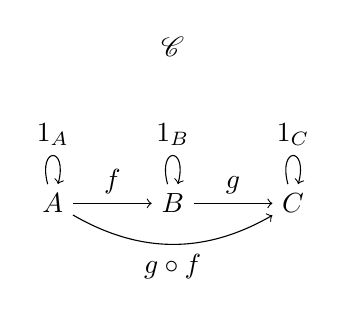
\begin{tikzpicture}
	\node (A) {$A$};
	\node [right=1cm of A] (B) {$B$};
	\node [right=1cm of B] (C) {$C$};
	\node [above=1.5cm of B] (catc) {$\cat{C}$};
	\draw [->] (A) to [edge label=$f$] (B);
	\draw [->] (B) to [edge label=$g$] (C);
	\draw [->, bend right] (A) to node [below] {$g\circ f$} (C);
	\draw [->, loop above] (A) to node [above] {$1_A$} (A);
	\draw [->, loop above] (B) to node [above] {$1_B$} (B);
	\draw [->, loop above] (C) to node [above] {$1_C$} (C);
\end{tikzpicture}
\end{document}
